\chapter{Further Gradient Estimations}
\label{section:moregradients}

\begin{figure}[h]
    \centering
    \begin{subfigure}[b]{0.47\textwidth}
        \centering
        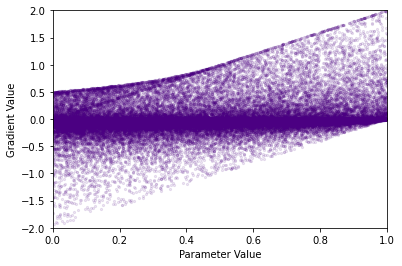
\includegraphics[width=\textwidth]{imgs/grad_prod_2_falseparam.png}
        \caption{Gradient samples for correct parameter $\F$}
        \label{fig:conjgrad2false}
    \end{subfigure}
    \begin{subfigure}[b]{0.47\textwidth}
        \centering
        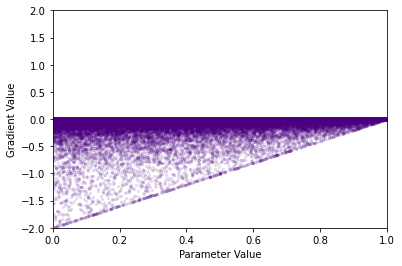
\includegraphics[width=\textwidth]{imgs/grad_prod_2_trueparam.png}
        \caption{Gradient samples for correct parameter $\T$}
        \label{fig:conjgrad2true}
    \end{subfigure}
    \begin{subfigure}[b]{0.47\textwidth}
        \centering
        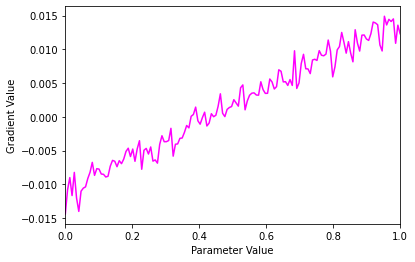
\includegraphics[width=\textwidth]{imgs/grad_prod_2_falseparam_avg.png}
        \caption{Mean gradient estimator for correct parameter $\F$}
        \label{fig:conjgrad2falseavg}
    \end{subfigure}
    \begin{subfigure}[b]{0.47\textwidth}
        \centering
        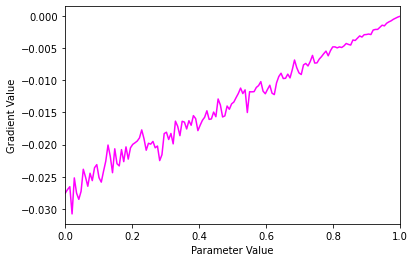
\includegraphics[width=\textwidth]{imgs/grad_prod_2_trueparam_avg.png}
        \caption{Mean gradient estimator for correct parameter $\T$}
        \label{fig:conjgrad2trueavg}
    \end{subfigure}
       \caption{Gradient estimations over the problem of real conjunctions with $\XOR$ loss $a=2$. We begin to see a separation between parameters, though the value of parameters with true value $\F$ seem to converge around 0.4, due to class imbalance.}
       \label{fig:conjgrad2}
\end{figure}

\begin{figure}[h]
    \centering
    \begin{subfigure}[b]{0.47\textwidth}
        \centering
        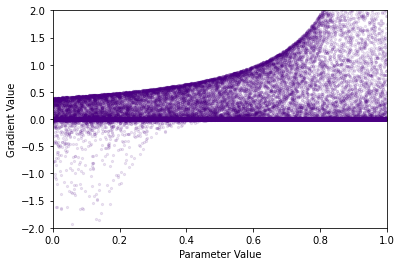
\includegraphics[width=\textwidth]{imgs/grad_prod_10_falseparam.png}
        \caption{Gradient samples for correct parameter $\F$}
        \label{fig:conjgrad10false}
    \end{subfigure}
    \begin{subfigure}[b]{0.47\textwidth}
        \centering
        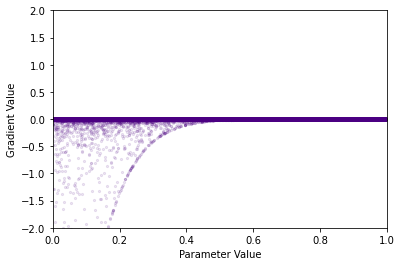
\includegraphics[width=\textwidth]{imgs/grad_prod_10_trueparam.png}
        \caption{Gradient samples for correct parameter $\T$}
        \label{fig:conjgrad10true}
    \end{subfigure}
    \begin{subfigure}[b]{0.47\textwidth}
        \centering
        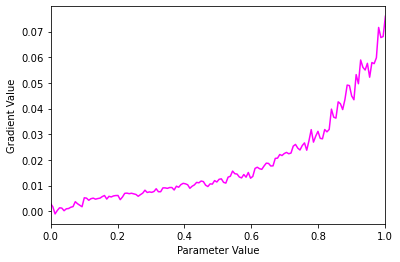
\includegraphics[width=\textwidth]{imgs/grad_prod_10_falseparam_avg.png}
        \caption{Mean gradient estimator for correct parameter $\F$}
        \label{fig:conjgrad10falseavg}
    \end{subfigure}
    \begin{subfigure}[b]{0.47\textwidth}
        \centering
        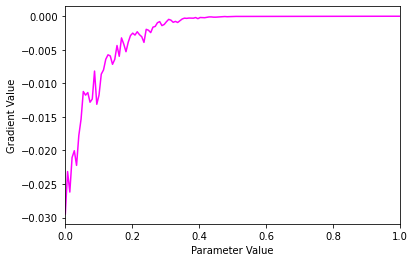
\includegraphics[width=\textwidth]{imgs/grad_prod_10_trueparam_avg.png}
        \caption{Mean gradient estimator for correct parameter $\T$}
        \label{fig:conjgrad10trueavg}
    \end{subfigure}
       \caption{Gradient estimations over the problem of real conjunctions with $\XOR$ loss $a=10$, Product logic, 10 dimensions. A much clearer separation between parameters.}
       \label{fig:conjgrad10}
\end{figure}


\begin{figure}[h]
    \centering
    \begin{subfigure}[b]{0.47\textwidth}
        \centering
        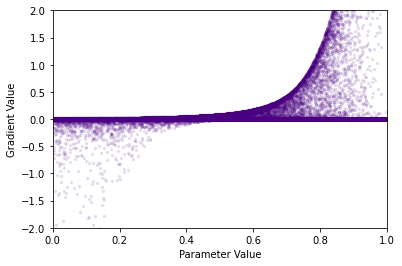
\includegraphics[width=\textwidth]{imgs/grad_ss_10_falseparam.png}
        \caption{Gradient samples for correct parameter $\F$}
        \label{fig:conjgrad10falsess}
    \end{subfigure}
    \begin{subfigure}[b]{0.47\textwidth}
        \centering
        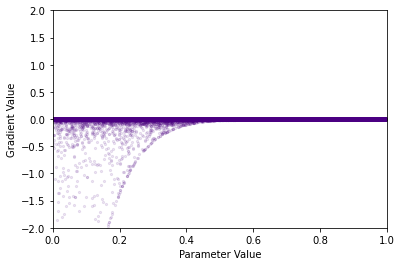
\includegraphics[width=\textwidth]{imgs/grad_ss_10_trueparam.png}
        \caption{Gradient samples for correct parameter $\T$}
        \label{fig:conjgrad10truess}
    \end{subfigure}
    \begin{subfigure}[b]{0.47\textwidth}
        \centering
        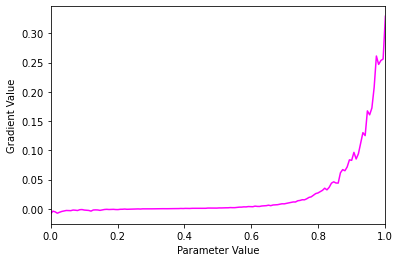
\includegraphics[width=\textwidth]{imgs/grad_ss_10_falseparam_avg.png}
        \caption{Mean gradient estimator for correct parameter $\F$}
        \label{fig:conjgrad10falseavgss}
    \end{subfigure}
    \begin{subfigure}[b]{0.47\textwidth}
        \centering
        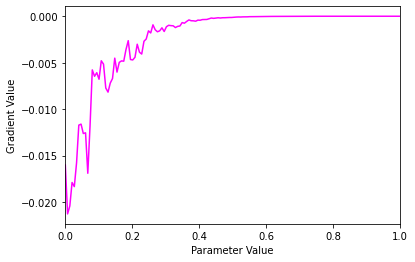
\includegraphics[width=\textwidth]{imgs/grad_ss_10_trueparam_avg.png}
        \caption{Mean gradient estimator for correct parameter $\T$}
        \label{fig:conjgrad10trueavgss}
    \end{subfigure}
       \caption{Gradient estimations over the problem of real conjunctions with $\XOR$ loss $a=10$, Schweizer-Sklar logic $p=-2$, 10 dimensions. Note that the size of the gradient estimator is an order of magnitude larger than Product logic for inferences.}
       \label{fig:conjgrad10ss}
\end{figure}

\begin{figure}[h]
    \centering
    \begin{subfigure}[b]{0.47\textwidth}
        \centering
        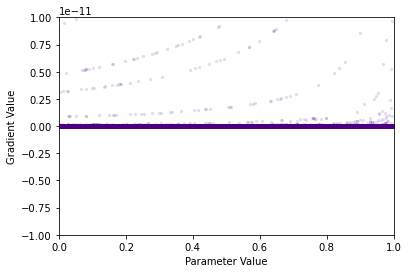
\includegraphics[width=\textwidth]{imgs/grad_prod_10_falseparam_100dim.png}
        \caption{Gradient samples for correct parameter $\F$}
        \label{fig:conjgrad10false100}
    \end{subfigure}
    \begin{subfigure}[b]{0.47\textwidth}
        \centering
        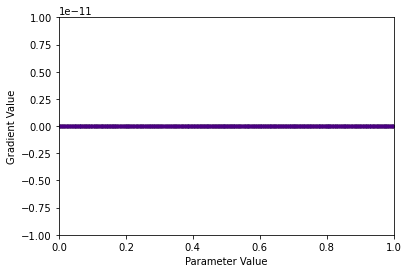
\includegraphics[width=\textwidth]{imgs/grad_prod_10_trueparam_100dim.png}
        \caption{Gradient samples for correct parameter $\T$}
        \label{fig:conjgrad10true100}
    \end{subfigure}
    \begin{subfigure}[b]{0.47\textwidth}
        \centering
        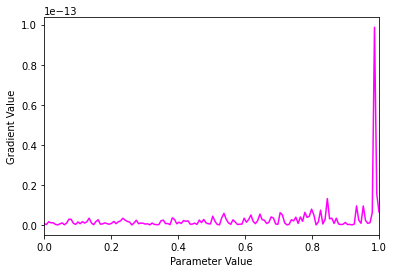
\includegraphics[width=\textwidth]{imgs/grad_prod_10_falseparam_100dim_avg.png}
        \caption{Mean gradient estimator for correct parameter $\F$}
        \label{fig:conjgrad10falseavg100}
    \end{subfigure}
    \begin{subfigure}[b]{0.47\textwidth}
        \centering
        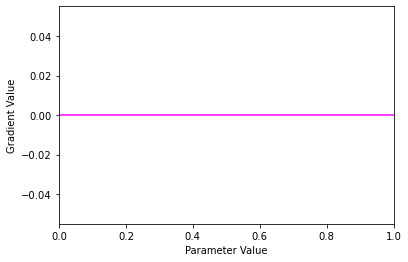
\includegraphics[width=\textwidth]{imgs/grad_prod_10_trueparam_100dim_avg.png}
        \caption{Mean gradient estimator for correct parameter $\T$}
        \label{fig:conjgrad10trueavg100}
    \end{subfigure}
       \caption{Gradient estimations over the problem of real conjunctions with $\XOR$ loss $a=10$, Product logic, 100 dimensions. A clear example of the curse of dimensionality applying to the vanishing gradient estimate.}
       \label{fig:conjgrad10100}
\end{figure}

\begin{figure}[h]
    \centering
    \begin{subfigure}[b]{0.47\textwidth}
        \centering
        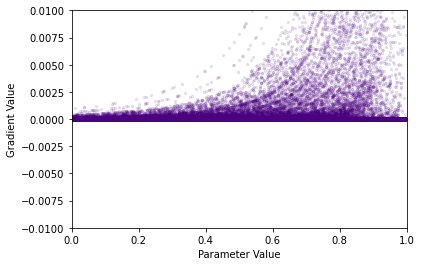
\includegraphics[width=\textwidth]{imgs/grad_ss_10_falseparam_100dim.png}
        \caption{Gradient samples for correct parameter $\F$}
        \label{fig:conjgrad10falsess100}
    \end{subfigure}
    \begin{subfigure}[b]{0.47\textwidth}
        \centering
        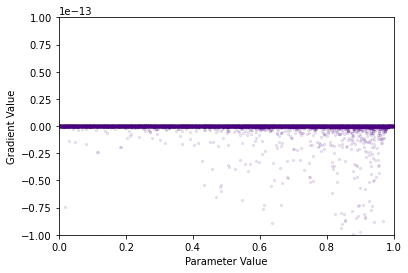
\includegraphics[width=\textwidth]{imgs/grad_ss_10_trueparam_100dim.png}
        \caption{Gradient samples for correct parameter $\T$}
        \label{fig:conjgrad10truess100}
    \end{subfigure}
    \begin{subfigure}[b]{0.47\textwidth}
        \centering
        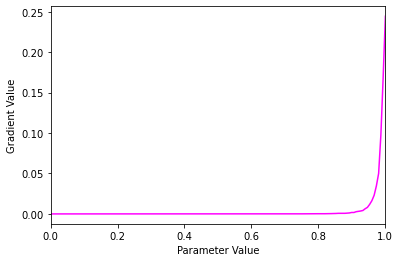
\includegraphics[width=\textwidth]{imgs/grad_ss_10_falseparam_100dim_avg.png}
        \caption{Mean gradient estimator for correct parameter $\F$}
        \label{fig:conjgrad10falseavgss100}
    \end{subfigure}
    \begin{subfigure}[b]{0.47\textwidth}
        \centering
        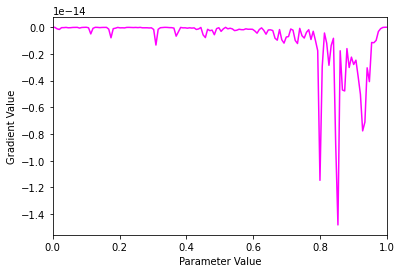
\includegraphics[width=\textwidth]{imgs/grad_ss_10_trueparam_100dim_avg.png}
        \caption{Mean gradient estimator for correct parameter $\T$}
        \label{fig:conjgrad10trueavgss100}
    \end{subfigure}
       \caption{Gradient estimations over the problem of real conjunctions with $\XOR$ loss $a=10$, Schweizer-Sklar logic $p=-2$, 100 dimensions. An example of Schweizer-Sklar logic being more adept against the curse of dimensionality, when making inferences.}
       \label{fig:conjgrad10ss100}
\end{figure}


\begin{figure}[h]
    \centering
    \begin{subfigure}[b]{0.47\textwidth}
        \centering
        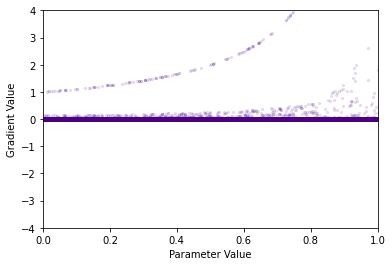
\includegraphics[width=\textwidth]{imgs/grad_prod_bce_falseparam_100dim.png}
        \caption{Gradient samples for correct parameter $\F$}
        \label{fig:conjgrad100falsebce}
    \end{subfigure}
    \begin{subfigure}[b]{0.47\textwidth}
        \centering
        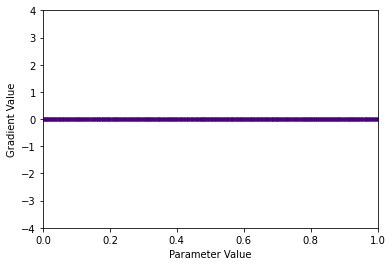
\includegraphics[width=\textwidth]{imgs/grad_prod_bce_trueparam_100dim.png}
        \caption{Gradient samples for correct parameter $\T$}
        \label{fig:conjgrad100truebce}
    \end{subfigure}
    \begin{subfigure}[b]{0.47\textwidth}
        \centering
        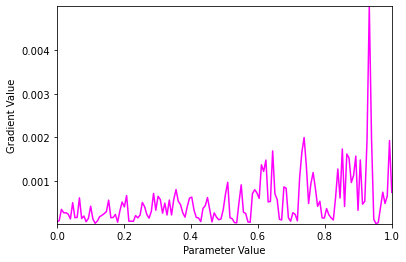
\includegraphics[width=\textwidth]{imgs/grad_prod_bce_falseparam_100dim_avg.png}
        \caption{Mean gradient estimator for correct parameter $\F$}
        \label{fig:conjgrad100falseavgbce}
    \end{subfigure}
    \begin{subfigure}[b]{0.47\textwidth}
        \centering
        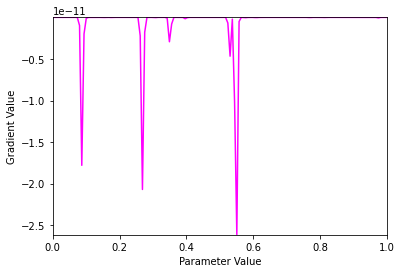
\includegraphics[width=\textwidth]{imgs/grad_prod_bce_trueparam_100dim_avg.png}
        \caption{Mean gradient estimator for correct parameter $\T$}
        \label{fig:conjgrad100trueavgbce}
    \end{subfigure}
       \caption{Gradient estimations over the problem of real conjunctions with binary cross-entropy loss, Product logic, 100 dimensions. Although improved over $\XOR$ loss, we still observe the curse of dimensionality.}
       \label{fig:conjgrad100bce}
\end{figure}

\begin{figure}[h]
    \centering
    \begin{subfigure}[b]{0.47\textwidth}
        \centering
        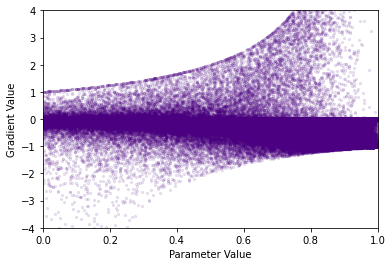
\includegraphics[width=\textwidth]{imgs/grad_ss_bce_falseparam_10dim.png}
        \caption{Gradient samples for correct parameter $\F$}
        \label{fig:conjgrad10falsessbce}
    \end{subfigure}
    \begin{subfigure}[b]{0.47\textwidth}
        \centering
        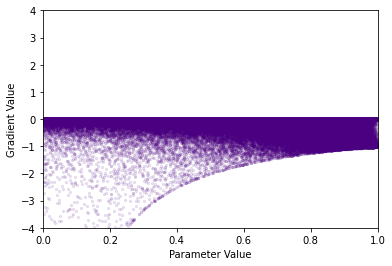
\includegraphics[width=\textwidth]{imgs/grad_ss_bce_trueparam_10dim.png}
        \caption{Gradient samples for correct parameter $\T$}
        \label{fig:conjgrad10truessbce}
    \end{subfigure}
    \begin{subfigure}[b]{0.47\textwidth}
        \centering
        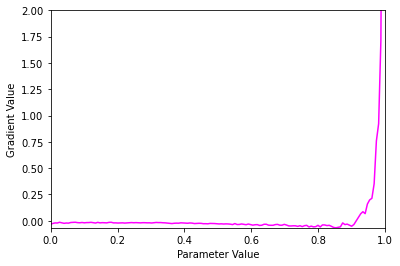
\includegraphics[width=\textwidth]{imgs/grad_ss_bce_falseparam_10dim_avg.png}
        \caption{Mean gradient estimator for correct parameter $\F$}
        \label{fig:conjgrad10falseavgssbce}
    \end{subfigure}
    \begin{subfigure}[b]{0.47\textwidth}
        \centering
        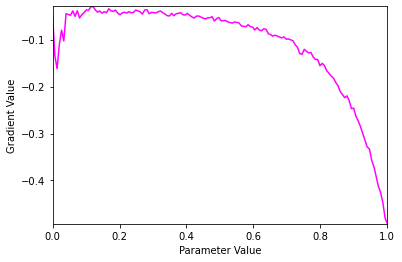
\includegraphics[width=\textwidth]{imgs/grad_ss_bce_trueparam_10dim_avg.png}
        \caption{Mean gradient estimator for correct parameter $\T$}
        \label{fig:conjgrad10trueavgssbce}
    \end{subfigure}
       \caption{Gradient estimations over the problem of real conjunctions with binary cross-entropy loss, Schweizer-Sklar logic $p=-2$, 10 dimensions. An even better separation of gradients.}
       \label{fig:conjgrad10ssbce}
\end{figure}

\begin{figure}[h]
    \centering
    \begin{subfigure}[b]{0.47\textwidth}
        \centering
        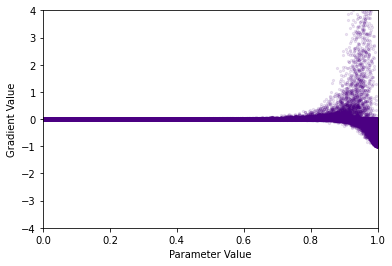
\includegraphics[width=\textwidth]{imgs/grad_ss_bce_falseparam_100dim.png}
        \caption{Gradient samples for correct parameter $\F$}
        \label{fig:conjgrad100falsessbce}
    \end{subfigure}
    \begin{subfigure}[b]{0.47\textwidth}
        \centering
        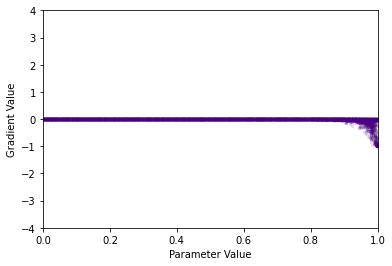
\includegraphics[width=\textwidth]{imgs/grad_ss_bce_trueparam_100dim.png}
        \caption{Gradient samples for correct parameter $\T$}
        \label{fig:conjgrad100truessbce}
    \end{subfigure}
    \begin{subfigure}[b]{0.47\textwidth}
        \centering
        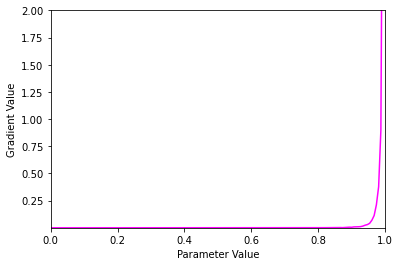
\includegraphics[width=\textwidth]{imgs/grad_ss_bce_falseparam_100dim_avg.png}
        \caption{Mean gradient estimator for correct parameter $\F$}
        \label{fig:conjgrad100falseavgssbce}
    \end{subfigure}
    \begin{subfigure}[b]{0.47\textwidth}
        \centering
        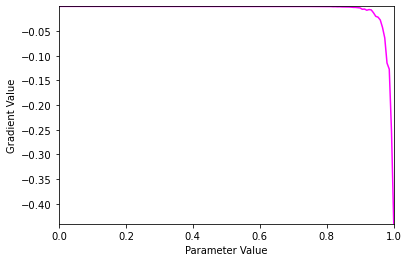
\includegraphics[width=\textwidth]{imgs/grad_ss_bce_trueparam_100dim_avg.png}
        \caption{Mean gradient estimator for correct parameter $\T$}
        \label{fig:conjgrad100trueavgssbce}
    \end{subfigure}
       \caption{Gradient estimations over the problem of real conjunctions with binary cross-entropy loss, Schweizer-Sklar logic $p=-2$, 100 dimensions. Note the magnitude of the gradients has not suffered much at all.}
       \label{fig:conjgrad100ssbce}
\end{figure}

\begin{figure}[h]
    \centering
    \begin{subfigure}[b]{0.47\textwidth}
        \centering
        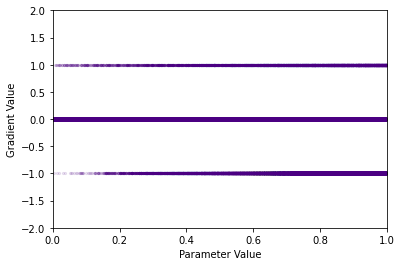
\includegraphics[width=\textwidth]{imgs/grad_min_1_falseparam.png}
        \caption{Gradient samples for correct parameter $\F$, $a=1$}
        \label{fig:conjgrad10falsem}
    \end{subfigure}
    \begin{subfigure}[b]{0.47\textwidth}
        \centering
        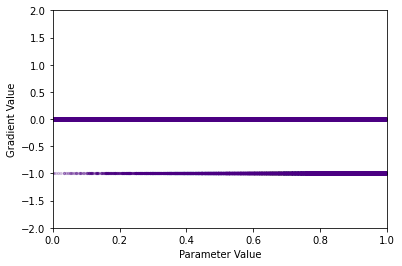
\includegraphics[width=\textwidth]{imgs/grad_min_1_trueparam.png}
        \caption{Gradient samples for correct parameter $\T$, $a=1$}
        \label{fig:conjgrad10truem}
    \end{subfigure}
    \begin{subfigure}[b]{0.47\textwidth}
        \centering
        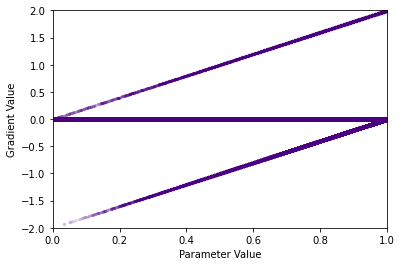
\includegraphics[width=\textwidth]{imgs/grad_min_2_falseparam.png}
        \caption{Gradient samples for correct parameter $\F$, $a=2$}
        \label{fig:conjgrad10falseavgm}
    \end{subfigure}
    \begin{subfigure}[b]{0.47\textwidth}
        \centering
        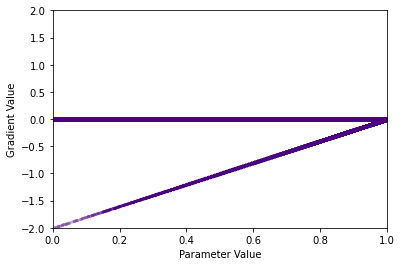
\includegraphics[width=\textwidth]{imgs/grad_min_2_trueparam.png}
        \caption{Gradient samples for correct parameter $\T$, $a=2$}
        \label{fig:conjgrad10trueavgm}
    \end{subfigure}
       \caption{Gradient estimations over the problem of real conjunctions under $\XOR$ loss with different exponents. Minimum logic, 10 dimensions. An example of binarization of gradient estimates.}
       \label{fig:conjgrad10m}
\end{figure}
